\chapter{Proximity Problems}
\label{ch:proximity}

\section{Closest Pair of Points}
\label{sec:closest_pair}

The closest pair of points problem is a fundamental challenge in computational geometry that involves finding the two points in a set of $n$ points that have the minimum Euclidean distance between them. While a naive brute-force approach takes $O(n^2)$ time, more efficient algorithms exist, including a deterministic $O(n \log n)$ divide-and-conquer approach by Shamos and Hoey~\cite{shamos1975} and Bentley and Shamos~\cite{bentley1976}, and a randomized $O(n)$ grid-based approach.

\subsection{Definitions}

\begin{definition}[Closest Pair]\label{def:closest_pair}
Given a set $P$ of $n$ points in $\mathbb{R}^2$, the \emph{closest pair} is the pair $(p_i, p_j)$ with $i \ne j$ that minimizes the Euclidean distance $\|p_i - p_j\|$.
\end{definition}

\begin{definition}[Euclidean Distance]\label{def:euclidean_distance}
For two points $P_1(x_1, y_1)$ and $P_2(x_2, y_2)$, the \emph{Euclidean distance}\index{Euclidean distance} is $d(P_1, P_2) = \sqrt{(x_2-x_1)^2 + (y_2-y_1)^2}$.
\end{definition}

\begin{definition}[Divide and Conquer Strategy]\label{def:dc_strategy}
A \emph{divide-and-conquer}\index{divide and conquer} strategy recursively partitions the input into two halves, solves each half independently, and merges the results. For the closest pair problem, the merge step requires examining only a narrow strip of width $2d$ centered on the dividing line, where $d = \min(d_L, d_R)$.
\end{definition}

\subsection{Theory}

\subsubsection*{Divide and Conquer Approach}

The set of points is first sorted by $x$-coordinate and then split into two halves by a vertical line. The minimum distance is recursively found in the left half ($d_L$) and the right half ($d_R$). Let $d = \min(d_L, d_R)$. The global minimum could still be a pair of points where one is in the left half and one is in the right half. To check this, we only need to consider points within a vertical ``strip'' of width $2d$ centered on the dividing line.

Within this strip, for any point $P$, we only need to check points $Q$ that are within distance $d$ of $P$. If the strip points are sorted by $y$-coordinate, it can be proven that each point only needs to be compared with a constant number (at most 7) of succeeding points in the sorted list to find a pair closer than $d$.

\begin{theorem}[Strip Lemma]\label{thm:strip_lemma}
Let $S$ be a set of points in a $2d \times d$ rectangle, sorted by $y$-coordinate. For each point $p \in S$, at most 7 other points in $S$ can lie within distance $d$ of $p$.
\end{theorem}
\begin{proof}
Divide the $2d \times d$ rectangle into 8 squares of side $d/2$. By the pigeonhole principle, if two points lie in the same square, their distance is at most $\frac{d}{2}\sqrt{2} < d$. However, each square can contain at most one point from a pair with mutual distance $\ge d$, giving at most 8 points total (including $p$). Thus $p$ needs to compare with at most 7 others.
\end{proof}

\begin{theorem}[Closest Pair Correctness]\label{thm:closest_pair_correctness}
The divide-and-conquer closest pair algorithm correctly finds the closest pair of $n$ points in $\mathbb{R}^2$.
\end{theorem}
\begin{proof}
By induction on $n$. The base cases ($n \le 3$) are solved by brute force. For the recursive case, the minimum distance is either entirely within the left half, entirely within the right half, or crosses the dividing line. The recursive calls find $d_L$ and $d_R$, and $d = \min(d_L, d_R)$. By the Strip Lemma (\cref{thm:strip_lemma}), only points within the strip need to be checked for a closer cross-pair, and the constant-bounded comparisons ensure no cross-pair closer than $d$ is missed.
\end{proof}

\subsubsection*{Randomized Grid Approach}

This approach uses a grid with cell size $d \times d$. Each cell in the grid contains at most one point (if $d$ is the current minimum distance). When a new point is added, we check its own cell and the 8 neighboring cells. If a closer point is found, the minimum distance $d$ is updated, and the grid is rebuilt with the new cell size. In the randomized version, the expected number of rebuilds is $O(\log n)$, leading to an overall expected time of $O(n)$.

\begin{figure}[htbp]
\centering
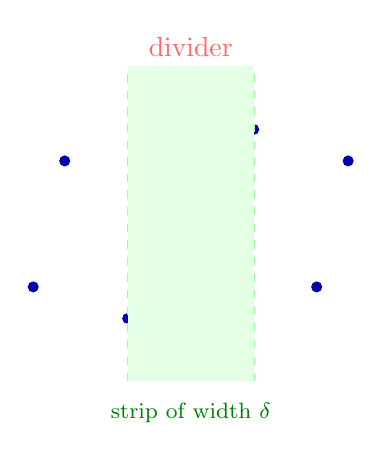
\begin{tikzpicture}[scale=0.8]
  \draw[red!60,thick,dashed] (3,-0.5)--(3,4.5) node[above] {divider};
  \fill[blue!70!black] (0.5,1) circle (2.5pt);
  \fill[blue!70!black] (1,3) circle (2.5pt);
  \fill[blue!70!black] (2,0.5) circle (2.5pt);
  \fill[blue!70!black] (2.5,2.5) circle (2.5pt);
  \fill[blue!70!black] (3.5,2) circle (2.5pt);
  \fill[blue!70!black] (4,3.5) circle (2.5pt);
  \fill[blue!70!black] (5,1) circle (2.5pt);
  \fill[blue!70!black] (5.5,3) circle (2.5pt);
  \draw[thick,orange] (2.5,2.5)--(3.5,2);
  \fill[orange] (2.5,2.5) circle (3pt);
  \fill[orange] (3.5,2) circle (3pt);
  \draw[green!40,thick,dashed] (2,-0.5)--(2,4.5);
  \draw[green!40,thick,dashed] (4,-0.5)--(4,4.5);
  \fill[green!10] (2,-0.5) rectangle (4,4.5);
  \node[font=\footnotesize,green!50!black] at (3,-1) {strip of width $\delta$};
\end{tikzpicture}
\caption{Closest pair: divide-and-conquer splits points along a vertical line. The closest pair may cross the dividing strip.}
\label{fig:closest_pair}
\end{figure}


\subsection{Pseudocode}

\begin{algorithm}[htbp]
\caption{Divide-and-Conquer Closest Pair}
\label{alg:closest_pair}
\begin{algorithmic}[1]
\Function{ClosestPair}{$points\_sorted\_x$, $points\_sorted\_y$}
  \If{$\text{len}(points\_sorted\_x) \le 3$}
    \State \Return $\text{BruteForce}(points\_sorted\_x)$
  \EndIf
  \State $mid \gets \text{len}(points\_sorted\_x) // 2$
  \State $left\_x \gets points\_sorted\_x[:mid]$
  \State $right\_x \gets points\_sorted\_x[mid:]$
  \State $(d\_L, p1\_L, p2\_L) \gets \text{ClosestPair}(left\_x, points\_sorted\_y\_left)$
  \State $(d\_R, p1\_R, p2\_R) \gets \text{ClosestPair}(right\_x, points\_sorted\_y\_right)$
  \State $d \gets \min(d\_L, d\_R)$
  \State $best\_pair \gets (p1\_L, p2\_L)$ if $d\_L < d\_R$ else $(p1\_R, p2\_R)$
  \State $strip \gets [p \mid p \in points\_sorted\_y \wedge |p.x - points\_sorted\_x[mid].x| < d]$
  \For{$i = 0$ \textbf{to} $\text{len}(strip) - 1$}
    \For{$j = i + 1$ \textbf{to} $\min(i + 8, \text{len}(strip)) - 1$}
      \If{$\text{dist}(strip[i], strip[j]) < d$}
        \State $d \gets \text{dist}(strip[i], strip[j])$
        \State $best\_pair \gets (strip[i], strip[j])$
      \EndIf
    \EndFor
  \EndFor
  \State \Return $(d, best\_pair)$
\EndFunction
\end{algorithmic}
\end{algorithm}

\subsection{Parameters}

\begin{itemize}
\item \textbf{Algorithm Choice}: Use D\&C for general-purpose deterministic results. Use Grid-based for massive streaming datasets where $O(n \log n)$ is too slow.
\item \textbf{Base Case}: Brute force for $n < 4$ to avoid excessive recursion overhead.
\end{itemize}

\subsection{Complexity}

\begin{itemize}
\item \textbf{Divide and Conquer}: $O(n \log n)$\index{time complexity!$O(n \log n)$} time, $O(n)$ space.
\item \textbf{Grid-based}: $O(n)$ expected time, $O(n)$ space.
\end{itemize}

\begin{example}[Closest Pair by Hand]\label{ex:closest_pair}
Consider $P = \{(0,0),\, (1,3),\, (2,2),\, (4,1),\, (5,4)\}$, sorted by $x$.
\begin{enumerate}
\item Split at $x = 2$: left $L = \{(0,0),(1,3),(2,2)\}$, right $R = \{(4,1),(5,4)\}$.
\item Recurse on $L$: brute force gives $d_L = \|(1,3)-(2,2)\| = \sqrt{2}$.
\item Recurse on $R$: brute force gives $d_R = \|(4,1)-(5,4)\| = \sqrt{10}$.
\item $d = \sqrt{2}$. Strip: points with $|x - 2| < \sqrt{2}$, i.e., $x \in (0.586, 3.414)$: $\{(1,3),(2,2)\}$.
\item Check strip pairs: only $(1,3)$ and $(2,2)$ at distance $\sqrt{2}$: no improvement.
\item Result: closest pair is $(1,3)$ and $(2,2)$ with distance $\sqrt{2} \approx 1.414$.
\end{enumerate}
\end{example}

\subsection{Usages}

\begin{itemize}
\item \textbf{Collision Detection}: Finding the two closest objects in a physics simulation.
\item \textbf{Cluster Analysis}: Identifying tight groupings of data points.
\item \textbf{Air Traffic Control}: Detecting potential collisions between aircraft.
\item \textbf{Bioinformatics}: Comparing molecular structures or sequences.
\end{itemize}

\subsection{Testing and Edge Cases}

\begin{itemize}
\item \textbf{Identical Points}: Points with the exact same coordinates (distance 0).
\item \textbf{Vertical/Horizontal alignment}: Points forming a perfect grid or line.
\item \textbf{Large Coordinates}: Precision issues with squared distances ($x^2 + y^2$) for very large $x, y$.
\item \textbf{Sparse vs.\ Dense}: Performance on points scattered far apart vs.\ points clustered tightly together.
\item \textbf{Verification}: Always compare with an $O(n^2)$ brute-force implementation for small inputs during testing.
\end{itemize}

\subsection{References}

\begin{itemize}
\item Shamos, M. I., \& Hoey, D. (1975). ``Closest-point problems''. IEEE FOCS.
\item Khuller, S., \& Matias, Y. (1995). ``A simple randomized sieve algorithm for the closest-pair problem''. Information and Computation.
\item Bentley, J. L., \& Shamos, M. I. (1976). ``Divide-and-conquer in multidimensional space''. ACM STOC.
\item Wikipedia: Closest pair of points problem.
\end{itemize}


\section{Proximity Queries}
\label{sec:proximity_queries}

Proximity queries are a class of geometric problems focused on finding the spatial relationships between objects, specifically their distances and relative positions. These queries answer questions like ``Which object is closest to this point?'', ``Are these two objects intersecting?'', or ``How far apart are these two shapes?'' Proximity queries are the foundation of collision detection, spatial data mining, and robotics.

\subsection{Definitions}

\begin{definition}[Nearest Neighbor]\label{def:nearest_neighbor}
Given a set $P \subseteq \mathbb{R}^d$ and a query point $q$, the \emph{nearest neighbor}\index{nearest neighbor} of $q$ in $P$ is the point $p^* \in P$ minimizing $\|q - p^*\|$.
\end{definition}

\begin{definition}[K-Nearest Neighbors]\label{def:knn}
The \emph{$k$-nearest neighbors}\index{k-nearest neighbors} of a query point $q$ in a set $P$ are the $k$ points of $P$ closest to $q$, ordered by distance.
\end{definition}

\subsection{Theory}

Proximity queries are categorized by the type of geometric objects involved:
\begin{enumerate}
\item \textbf{Point-Point}: Handled using \textbf{KD-Trees}\index{KD-tree}~\cite{bentley1975} or \textbf{Quadtrees} for efficient $O(\log n)$ retrieval.
\item \textbf{Point-Mesh}: Finding the closest point on a surface. This involves searching a spatial index (like an \textbf{AABB Tree} or \textbf{BVH}) and calculating the distance to each triangle in the candidate leaves.
\item \textbf{Mesh-Mesh}: Calculating the distance between two 3D models. The \textbf{GJK (Gilbert-Johnson-Keerthi)} algorithm is the standard for convex shapes, while BVH hierarchies are used for general non-convex meshes.
\item \textbf{All-Pairs}: Finding all pairs of objects within a distance $r$. This is solved using \textbf{Spatial Hashing} or sweep-line algorithms.
\end{enumerate}

The efficiency of these queries relies heavily on \textbf{Spatial Partitioning} (dividing the space) or \textbf{Bounding Volume Hierarchies} (grouping the objects).

\begin{theorem}[KD-Tree Nearest Neighbor]\label{thm:kdtree_nn}
A KD-tree built on $n$ points in $\mathbb{R}^d$ supports nearest neighbor queries in $O(n^{1-1/d})$ worst-case time.
\end{theorem}

\subsection{Pseudocode}

\begin{algorithm}[htbp]
\caption{BVH Distance Query}
\label{alg:bvh_distance}
\begin{algorithmic}[1]
\Function{Distance}{nodeA, nodeB, current\_min}
  \If{$\text{BoxDistance}(nodeA.bbox, nodeB.bbox) \ge current\_min$}
    \State \Return $current\_min$
  \EndIf
  \If{$nodeA.\text{is\_leaf}$ \textbf{and} $nodeB.\text{is\_leaf}$}
    \For{$primA$ in $nodeA.primitives$}
      \For{$primB$ in $nodeB.primitives$}
        \State $d \gets \text{PrimitiveDistance}(primA, primB)$
        \State $current\_min \gets \min(current\_min, d)$
      \EndFor
    \EndFor
    \State \Return $current\_min$
  \EndIf
  \If{$nodeA.volume > nodeB.volume$}
    \For{$childA$ in $nodeA.children$}
      \State $current\_min \gets \text{Distance}(childA, nodeB, current\_min)$
    \EndFor
  \Else
    \For{$childB$ in $nodeB.children$}
      \State $current\_min \gets \text{Distance}(nodeA, childB, current\_min)$
    \EndFor
  \EndIf
  \State \Return $current\_min$
\EndFunction
\end{algorithmic}
\end{algorithm}

\subsection{Parameters}

\begin{itemize}
\item \textbf{Bounding Volume Type}: \textbf{AABB}\index{AABB} (fast intersection), \textbf{OOBB} (tighter fit), or \textbf{Bounding Spheres} (rotation invariant).
\item \textbf{Spatial Index}: Use \textbf{KD-Trees} for static points and \textbf{R-Trees}\index{R-tree} or \textbf{BVHs} for moving objects.
\end{itemize}

\subsection{Complexity}

\begin{itemize}
\item \textbf{Point NN}: $O(\log n)$ average using KD-Trees. $O(n^{1-1/d})$ worst case in $d$ dimensions~\cite{bentley1975}.
\item \textbf{Closest Pair}: $O(n \log n)$ deterministic or $O(n)$ randomized.
\item \textbf{Collision Detection}: $O(n \log n)$ for broad-phase, $O(1)$ for narrow-phase (convex primitives).
\end{itemize}

\subsection{Usages}

\begin{itemize}
\item \textbf{Physics Engines}: Real-time collision detection in video games (e.g., PhysX, Bullet).
\item \textbf{Machine Learning}: Clustering (K-Means) and classification (KNN).
\item \textbf{Robotics}: Obstacle avoidance and sensor fusion.
\item \textbf{Molecular Modeling}: Detecting van der Waals overlaps between atoms.
\item \textbf{GIS}: Finding the nearest points of interest (e.g., hospitals or fire stations).
\end{itemize}

\subsection{Testing and Edge Cases}

\begin{itemize}
\item \textbf{Identical Objects}: Distance should be zero.
\item \textbf{Touching Objects}: Distance should be zero or very small.
\item \textbf{Nested Objects}: Ensure the algorithm detects if one object is entirely inside another.
\item \textbf{Large Aspect Ratios}: Test with very long and thin objects which can ``leak'' through poorly fitted bounding volumes.
\item \textbf{Precision}: Verify distances for objects separated by many orders of magnitude.
\end{itemize}

\subsection{References}

\begin{itemize}
\item Gilbert, E. G., Johnson, D. W., \& Keerthi, S. S. (1988). ``A fast procedure for computing the distance between complex objects in three-dimensional space''. IEEE Journal on Robotics and Automation.
\item Ericson, C. (2004). ``Real-Time Collision Detection''. Morgan Kaufmann.
\item Samet, H. (2006). ``Foundations of Multidimensional and Metric Data Structures''. Elsevier.
\item Wikipedia: Nearest neighbor search.
\end{itemize}

\section{Industrial Applications of Nearest Neighbor Search}
\label{sec:nn_applications}

Nearest neighbor search (NNS)---finding the stored point closest to a query
point, or its $k$-nearest generalization of Definition~\ref{def:knn}---is the
most frequently used geometric primitive in industry because a surprising
number of problems reduce to ``find the most similar known item.'' The data
structures of Sections~\ref{sec:kd_tree} and \ref{sec:fixed_radius_search}
(and, for high dimensions, locality-sensitive hashing) make it practical at
billions of points~\cite{bentley1975,samet2006}. The following are the
principal industrial use cases.

\begin{itemize}
\item \textbf{Recommendation Systems}: Annoy was built at \texttt{Spotify}
  specifically for music recommendations---millions of tracks and users in a
  low-dimensional embedding space, queried for similar items---and the same
  nearest-neighbor formulation powers the recommendation engines of the
  largest web platforms.

\item \textbf{Semantic Search and Vector Databases}: Embedding-based
  semantic search is served by approximate nearest-neighbor (ANNS) indexes
  (HNSW, FAISS, DiskANN) at the core of commercial vector databases
  (Pinecone, Weaviate, Qdrant, Milvus, Elasticsearch kNN), a market sold to
  enterprise search, retrieval-augmented generation, and
  chatbot deployments~\cite{malkov2018}.

\item \textbf{Reverse Image and Visual Search}: Content-based retrieval
  encodes images (or frames) into embedding vectors and returns the $k$ most
  visually similar items by nearest-neighbor search in the embedding space,
  powering reverse image search, product visual search, and duplicate
  detection in retail and content platforms.

\item \textbf{Geospatial Services}: Mapping, ride-hailing, and navigation
  apps answer ``closest restaurant'' or ``nearest pickup point'' through
  spatial nearest-neighbor queries over point-of-interest databases
  (Section~\ref{sec:kd_tree}), a query type materialized at billion-query
  scale by location platforms.

\item \textbf{Autonomous Driving and Robotics}: Nearest-neighbor search over
  a precomputed point cloud aligns sensor scans (point-cloud registration,
  ICP), matches features for SLAM loop closure, and finds the nearest
  obstacle for collision checking and path planning in commercial
  autonomous-driving and robotics stacks.

\item \textbf{Drug Discovery and Molecular Similarity}: Molecular similarity
  by fingerprints or descriptors is a nearest-neighbor query over compound
  databases, used to find the closest known active molecule to a candidate
  drug; structure- and ligand-based virtual screening is sold commercially
  by computational-chemistry vendors.

\item \textbf{Fraud Detection and Anomaly Detection}: Transactions embedded
  into a feature space are flagged when their nearest neighbors are
  predominantly fraudulent or when the distance to all known-good neighbors
  exceeds a learned threshold---an anomaly-detection formulation of NNS
  shipped in commercial fraud and security analytics platforms.

\item \textbf{Bioinformatics and Genomics}: DNA and protein sequences
  compared by edit distance use nearest-neighbor search over a string-space
  index to find the closest gene, detect homology, and cluster metagenomic
  samples, powering commercial sequencing-analysis pipelines.

\item \textbf{Pattern Recognition and Classification}: The k-nearest
  neighbors classifier (k-NN) labels a query point by the majority class of
  its $k$ nearest training points; it remains a production baseline in
  biometric identification, OCR, and spam filtering.
\end{itemize}

\subsection{Industrial-Scale Software}
Exact and approximate NNS is implemented in \texttt{scipy.spatial.cKDTree}
(KD-tree), \texttt{FLANN} and \texttt{FAISS} (approximate, billion-scale),
\texttt{HNSWlib} (graph-based ANNS), \texttt{Annoy} (random-projection
forests), and \texttt{PostGIS} (spatial nearest-neighbor SQL), in addition to
the KD-tree and fixed-radius structures of
Sections~\ref{sec:kd_tree} and \ref{sec:fixed_radius_search}~\cite{malkov2018}.


\section{Range Search}
\label{sec:range_search}

Range searching\index{range search} is a fundamental task in computational geometry where the goal is to efficiently retrieve all geometric objects (typically points) that lie within a specified query region (the ``range''). Query regions are usually simple shapes like axis-aligned rectangles (orthogonal range search), circles, or half-planes. Efficient range searching is the backbone of spatial databases, geographic information systems (GIS), and computer graphics. Foundational work on range search data structures was done by Bentley~\cite{bentley1975} and Lueker~\cite{lueker1978}.

\subsection{Definitions}

\begin{definition}[Range Search]\label{def:range_search}
Given a set $P$ of $n$ points in $\mathbb{R}^d$ and a query region $R$, the \emph{range search} problem asks to either report all points $p \in P \cap R$ (range reporting) or count $|P \cap R|$ (range counting).
\end{definition}

\begin{definition}[Orthogonal Range Query]\label{def:orthogonal_range}
An \emph{orthogonal range query}\index{orthogonal range query} is a range search where the query region is an axis-aligned hyper-rectangle $R = [x_1, x_2] \times [y_1, y_2] \times \cdots$.
\end{definition}

\subsection{Theory}

The efficiency of range search depends on the dimensionality and the type of range.
\begin{enumerate}
\item \textbf{1D Range Search}: Solved using a balanced binary search tree in $O(\log n + k)$ time.
\item \textbf{Orthogonal Range Search ($d$-dimensions)}:
  \begin{itemize}
  \item \textbf{KD-Trees}: Good for medium dimensions; $O(\sqrt{n} + k)$ query time in 2D.
  \item \textbf{Range Trees}\index{range tree}: Faster query time $O(\log^d n + k)$ but higher space $O(n \log^{d-1} n)$.
  \item \textbf{Quadtrees}: Effective for non-uniform data distributions.
  \end{itemize}
\item \textbf{Circular/Spherical Range Search}: Often handled using KD-trees with a distance-based pruning condition or specialized structures like \textbf{Ball Trees}.
\item \textbf{Non-Orthogonal Range Search}: General shapes can be approximated by rectangles or handled using more complex structures like \textbf{Simplex Range Reporting}.
\end{enumerate}

The fundamental tradeoff in range search is between \textbf{Query Time}, \textbf{Preprocessing Time}, and \textbf{Space Complexity}.

\begin{theorem}[Range Tree Query Time]\label{thm:range_tree}
A range tree on $n$ points in $\mathbb{R}^d$ uses $O(n \log^{d-1} n)$ space and supports orthogonal range reporting queries in $O(\log^d n + k)$ time, where $k$ is the number of reported points.
\end{theorem}

\subsection{Pseudocode}

\begin{algorithm}[htbp]
\caption{Orthogonal Range Search (Tree-based)}
\label{alg:range_search}
\begin{algorithmic}[1]
\Function{RangeSearch}{node, query\_range, results}
  \If{$node$ is None}
    \State \Return
  \EndIf
  \If{$\neg\, \text{Intersect}(node.bbox, query\_range)$}
    \State \Return
  \EndIf
  \If{$\text{FullyContains}(query\_range, node.bbox)$}
    \State $results.\text{extend}(node.all\_points)$
    \State \Return
  \EndIf
  \If{$node.\text{is\_leaf}$}
    \For{$p$ in $node.points$}
      \If{$query\_range.\text{contains}(p)$}
        \State $results.\text{append}(p)$
      \EndIf
    \EndFor
  \Else
    \For{$child$ in $node.children$}
      \State $\text{RangeSearch}(child, query\_range, results)$
    \EndFor
  \EndIf
\EndFunction
\end{algorithmic}
\end{algorithm}

\subsection{Parameters}

\begin{itemize}
\item \textbf{Dimensionality}: For $d > 20$, most spatial data structures degrade to linear search (the ``Curse of Dimensionality'').
\item \textbf{Data Distribution}: Use \textbf{Quadtrees} or \textbf{R-Trees} for highly clustered data; use \textbf{KD-Trees} or \textbf{Range Trees} for more uniform data.
\item \textbf{Memory}: If memory is tight, KD-trees are preferred ($O(n)$ space).
\end{itemize}

\subsection{Complexity Summary}

\begin{center}
\begin{tabular}{|l|c|c|}
\hline
\textbf{Structure} & \textbf{Space} & \textbf{Query (2D Reporting)} \\
\hline
KD-Tree & $O(n)$ & $O(\sqrt{n} + k)$ \\
Range Tree & $O(n \log n)$ & $O(\log^2 n + k)$ \\
Quadtree & $O(depth \cdot n)$ & $O(depth + k)$ \\
R-Tree & $O(n)$ & $O(\log n + k)$ (avg) \\
\hline
\end{tabular}
\end{center}

\subsection{Usages}

\begin{itemize}
\item \textbf{Spatial Databases}: Finding all customers within a specific zip code or radius.
\item \textbf{Computer Graphics}: Frustum culling and identifying all objects hit by a blast radius.
\item \textbf{GIS}: Overlaying different map layers (e.g., finding all houses in a flood zone).
\item \textbf{Machine Learning}: Preprocessing for K-Nearest Neighbors (KNN).
\item \textbf{Collision Detection}: Finding all pairs of objects that might be colliding.
\end{itemize}

\begin{example}[1D Range Search]\label{ex:1d_range}
Given sorted points $P = \{1, 3, 5, 7, 9, 11, 13\}$ and query range $R = [4, 10]$, a binary search locates the first point $\ge 4$ (which is 5) and the last point $\le 10$ (which is 9). All points in this contiguous subsequence $\{5, 7, 9\}$ are returned in $O(\log n + k)$ time, where $k = 3$.
\end{example}

\subsection{Testing and Edge Cases}

\begin{itemize}
\item \textbf{Empty Query}: Ensure the algorithm returns an empty list for a range containing no points.
\item \textbf{Full Range Query}: Verify that a range covering the entire domain returns all $n$ points.
\item \textbf{Points on Boundaries}: Consistently handle points exactly on the edge of the query rectangle.
\item \textbf{Overlapping Points}: Ensure duplicate points are correctly counted/reported.
\item \textbf{Very Large Coordinates}: Precision check for queries far from the origin.
\end{itemize}

\subsection{References}

\begin{itemize}
\item Bentley, J. L. (1975). ``Multidimensional binary search trees used for associative searching''. Communications of the ACM.
\item Lueker, G. S. (1978). ``A data structure for orthogonal range queries''. IEEE FOCS.
\item Berg, M. de, Cheong, O., Kreveld, M. van, \& Overmars, M. (2008). ``Computational Geometry: Algorithms and Applications''. Springer-Verlag.
\item Wikipedia: Range searching.
\end{itemize}


\section{Point in Polygon (Winding Number)}
\label{sec:point_in_polygon_winding}

The Winding Number algorithm\index{winding number} is a robust method for determining whether a point lies inside a given polygon. It calculates the total number of times the polygon's boundary wraps around the test point. A winding number of zero indicates the point is outside the polygon, while a non-zero value indicates it is inside. This method is particularly superior to the Ray Casting algorithm when dealing with self-intersecting polygons. Analysis of the winding number method for arbitrary polygons is given by Sunday~\cite{sunday2001} and H\"{o}rmann and Agathos~\cite{hormann2001}.

\subsection{Definitions}

\begin{definition}[Winding Number]\label{def:winding_number}
The \emph{winding number}\index{winding number} $wn(P, C)$ of a point $P$ with respect to a closed curve $C$ is the total number of times $C$ winds counter-clockwise around $P$. Formally, it equals $\frac{1}{2\pi} \oint_C d\theta$ where $\theta$ is the angle from $P$ to a point on $C$.
\end{definition}

\begin{definition}[Is-Left Test]\label{def:is_left}
The \emph{Is-Left test} determines whether a point $P$ is to the left of the directed line from $V_1$ to $V_2$:
\[
\operatorname{IsLeft}(V_1, V_2, P) = (V_2.x - V_1.x)(P.y - V_1.y) - (P.x - V_1.x)(V_2.y - V_1.y).
\]
This is equivalent to the signed area of $\triangle V_1 V_2 P$ (up to a factor of 2).
\end{definition}

\subsection{Theory}

The algorithm counts the net number of full revolutions the polygon makes around the point $P$. As we traverse the polygon's edges:
\begin{itemize}
\item Every time an edge crosses the positive $x$-ray of $P$ going \textbf{upward}, we increment the winding number.
\item Every time an edge crosses the positive $x$-ray of $P$ going \textbf{downward}, we decrement the winding number.
\end{itemize}

Crucially, an edge is only counted if the point $P$ is actually to the left of the upward edge (or to the right of the downward edge), ensuring that the crossing actually ``wraps'' around the point.

\begin{theorem}[Winding Number Correctness]\label{thm:winding_correctness}
A point $P$ lies inside a simple polygon $C$ if and only if $wn(P, C) \ne 0$. More precisely, the winding number counts the number of times $C$ encircles $P$.
\end{theorem}
\begin{proof}
The winding number is a topological invariant related to the degree of the map $\theta: C \to S^1$ defined by $\theta(q) = \frac{q - P}{\|q - P\|}$. By the Jordan Curve Theorem, for a simple closed curve, $wn(P, C) = \pm 1$ for interior points and $0$ for exterior points. The sign depends on the orientation of $C$. The incremental counting algorithm correctly tracks the accumulated angle by detecting upward and downward crossings of the horizontal ray from $P$.
\end{proof}

\subsection{Pseudocode}

\begin{algorithm}[htbp]
\caption{Point-in-Polygon via Winding Number}
\label{alg:winding_number}
\begin{algorithmic}[1]
\Function{PointWindingNumber}{$P$, polygon}
  \State $wn \gets 0$
  \For{each edge $(V1, V2)$ in polygon}
    \If{$V1.y \le P.y$}
      \If{$V2.y > P.y$}
        \If{$\text{IsLeft}(V1, V2, P) > 0$}
          \State $wn \gets wn + 1$
        \EndIf
      \EndIf
    \Else
      \If{$V2.y \le P.y$}
        \If{$\text{IsLeft}(V1, V2, P) < 0$}
          \State $wn \gets wn - 1$
        \EndIf
      \EndIf
    \EndIf
  \EndFor
  \State \Return $wn$
\EndFunction

\Function{IsLeft}{$V1$, $V2$, $P$}
  \State \Return $(V2.x - V1.x) * (P.y - V1.y) - (P.x - V1.x) * (V2.y - V1.y)$
\EndFunction
\end{algorithmic}
\end{algorithm}

\subsection{Parameters}

\begin{itemize}
\item \textbf{Input}: A test \texttt{Point2D} and a list of \texttt{Point2D} vertices representing the polygon.
\item \textbf{Winding Rule}: Most applications use the \textbf{Non-Zero Winding Rule}\index{non-zero winding rule} (inside if $wn \ne 0$), though some use the \textbf{Odd-Even Rule} ($wn$ is odd).
\end{itemize}

\subsection{Complexity}

\begin{itemize}
\item \textbf{Time Complexity}: $O(n)$ where $n$ is the number of vertices. Each edge is visited exactly once.
\item \textbf{Space Complexity}: $O(1)$ auxiliary space, assuming the polygon vertices are already stored.
\end{itemize}

\begin{example}[Winding Number for a Square]\label{ex:winding_square}
Consider the unit square with vertices $(0,0), (1,0), (1,1), (0,1)$ traversed counter-clockwise. Testing point $P = (0.5, 0.5)$:
\begin{enumerate}
\item Edge $(0,0) \to (1,0)$: $V1.y = 0 \le 0.5$, $V2.y = 0 \not> 0.5$: no crossing.
\item Edge $(1,0) \to (1,1)$: $V1.y = 0 \le 0.5$, $V2.y = 1 > 0.5$: upward crossing. $\operatorname{IsLeft} = (1-1)(0.5-0) - (0.5-1)(1-0) = 0 + 0.5 = 0.5 > 0$: $wn \gets 1$.
\item Edge $(1,1) \to (0,1)$: $V1.y = 1 \not\le 0.5$: downward branch. $V2.y = 1 \not\le 0.5$: no crossing.
\item Edge $(0,1) \to (0,0)$: $V1.y = 1 \not\le 0.5$: downward branch. $V2.y = 0 \le 0.5$: downward crossing. $\operatorname{IsLeft} = (0-0)(0.5-1) - (0.5-0)(0-1) = 0 + 0.5 = 0.5 > 0$, but we need $< 0$: not counted (this is correct since the edge goes down and $P$ is to its right).
\end{enumerate}
Final $wn = 1 \ne 0$: point is inside. For $P = (2, 0.5)$ (outside), no crossings contribute: $wn = 0$.
\end{example}

\subsection{Usages}

\begin{itemize}
\item \textbf{SVG/PostScript Rendering}: Determining which areas of a complex path should be filled.
\item \textbf{GIS Analysis}: Checking if a GPS coordinate falls within a specific territorial boundary.
\item \textbf{Video Games}: Hitbox detection for complex, non-convex characters or objects.
\end{itemize}

\subsection{Testing and Edge Cases}

\begin{itemize}
\item \textbf{Point on Edge/Vertex}: The algorithm's behavior on the boundary depends on the strictness of the inequalities ($<$ vs $\le$).
\item \textbf{Horizontal Edges}: Handled correctly because they fail both the $V1.y \le P.y < V2.y$ and $V2.y \le P.y < V1.y$ conditions.
\item \textbf{Self-intersecting Polygons}: A ``figure-eight'' polygon will have regions with winding numbers of 1, $-1$, and 0.
\item \textbf{Degenerate Polygons}: Polygons with fewer than 3 vertices or zero area.
\end{itemize}

\subsection{References}

\begin{itemize}
\item Sunday, D. (2001). ``Inclusion of a Point in a Polygon''. Journal of Graphics Tools.
\item H\"{o}rmann, K., \& Agathos, A. (2001). ``The point in polygon problem for arbitrary polygons''. Computational Geometry.
\item Wikipedia: Point in polygon.
\end{itemize}


\section{Largest Empty Circle}
\label{sec:largest_empty_circle}

The largest empty circle problem asks for the circle of maximum radius whose center is within the convex hull of a given set of points $P$, and whose interior contains no points from $P$. This problem is a fundamental challenge in computational geometry with direct applications in facility location and urban planning.

\subsection{Definitions}

\begin{definition}[Largest Empty Circle]\label{def:largest_empty_circle}
Given a set $P \subseteq \mathbb{R}^2$, the \emph{largest empty circle} is the circle $C^*$ with maximum radius $r^*$ such that $C^*$ contains no point of $P$ in its interior and its center lies within $\operatorname{conv}(P)$.
\end{definition}

\subsection{Theory}

The largest empty circle must have its center at one of two types of locations:
\begin{enumerate}
\item \textbf{Voronoi Vertices}\index{Voronoi vertex}: A Voronoi vertex is the circumcenter of three points from $P$. If this vertex is inside the convex hull, it defines an empty circle passing through those three points.
\item \textbf{Intersection of Voronoi Edges and Convex Hull}: The center could be at the intersection of a Voronoi edge and an edge of the convex hull.
\end{enumerate}

The algorithm for finding the largest empty circle is:
\begin{enumerate}
\item Compute the \textbf{Voronoi Diagram} (\cref{alg:voronoi}) of the points $P$.
\item Iterate through all Voronoi vertices. For each vertex inside the convex hull, calculate the distance to its closest point (its radius).
\item Iterate through all intersections of Voronoi edges with the convex hull boundary. For each intersection, calculate the radius of the empty circle centered there.
\item The largest of all these radii defines the largest empty circle.
\end{enumerate}

\begin{theorem}[Optimality of Voronoi Vertices]\label{thm:lec_optimality}
The center of the largest empty circle of a point set $P$ in general position is either a Voronoi vertex of $P$ or lies on the intersection of a Voronoi edge with the boundary of $\operatorname{conv}(P)$.
\end{theorem}

\subsection{Pseudocode}

\begin{algorithm}[htbp]
\caption{Largest Empty Circle}
\label{alg:largest_empty_circle}
\begin{algorithmic}[1]
\Function{LargestEmptyCircle}{points}
  \State $CH \gets \text{ConvexHull}(points)$
  \State $VD \gets \text{Voronoi}(points)$
  \State $max\_radius \gets 0$
  \State $best\_center \gets \text{None}$
  \For{$v$ in $VD.vertices$}
    \If{$\text{PointInPolygon}(v, CH)$}
      \State $r \gets \text{Distance}(v, VD.\text{GetClosestSite}(v))$
      \If{$r > max\_radius$}
        \State $max\_radius \gets r$
        \State $best\_center \gets v$
      \EndIf
    \EndIf
  \EndFor
  \For{$edge$ in $VD.edges$}
    \For{$ch\_edge$ in $CH.edges$}
      \State $p \gets \text{Intersect}(edge, ch\_edge)$
      \If{$p$ is not None}
        \State $r \gets \text{Distance}(p, VD.\text{GetClosestSite}(p))$
        \If{$r > max\_radius$}
          \State $max\_radius \gets r$
          \State $best\_center \gets p$
        \EndIf
      \EndIf
    \EndFor
  \EndFor
  \State \Return $best\_center, max\_radius$
\EndFunction
\end{algorithmic}
\end{algorithm}

\subsection{Parameters}

\begin{itemize}
\item \textbf{Precision}: Finding the intersection of Voronoi edges and the convex hull requires careful handling of floating-point inaccuracies.
\item \textbf{Region Constraint}: The problem can be generalized to find the largest empty circle within any bounding polygon (not just the convex hull).
\end{itemize}

\subsection{Complexity}

\begin{itemize}
\item \textbf{Time Complexity}: $O(n \log n)$ to build the Voronoi diagram and convex hull. Finding intersections takes $O(n \log n)$ or $O(n)$ depending on the implementation.
\item \textbf{Space Complexity}: $O(n)$ to store the Voronoi and convex hull structures.
\end{itemize}

\subsection{Usages}

\begin{itemize}
\item \textbf{Facility Location}: Finding the location for a new facility (e.g., a toxic waste dump or a new shopping center) that is as far as possible from all existing points of interest.
\item \textbf{Urban Planning}: Determining where to place a new park to maximize the distance from the nearest noise sources.
\item \textbf{Robotics}: Path planning to stay as far from obstacles as possible (the ``safest'' path follows Voronoi edges).
\item \textbf{Signal Coverage}: Identifying the largest ``blind spot'' in a cellular or Wi-Fi network.
\end{itemize}

\subsection{Testing and Edge Cases}

\begin{itemize}
\item \textbf{Square/Rectangle Alignment}: For four points in a square, the center should be at the centroid.
\item \textbf{Points on a Circle}: All Voronoi vertices should coincide at the center of the circle.
\item \textbf{Collinear Points}: The convex hull is a line segment, so the circle will have zero radius.
\item \textbf{Sparse vs.\ Dense}: Ensure the algorithm handles large empty spaces correctly.
\item \textbf{Large Coordinates}: Precision check for very large $x, y$.
\end{itemize}

\subsection{References}

\begin{itemize}
\item Shamos, M. I., \& Hoey, D. (1975). ``Closest-point problems''. IEEE FOCS.
\item Preparata, F. P., \& Shamos, M. I. (1985). ``Computational Geometry: An Introduction''. Springer-Verlag.
\item Wikipedia: Largest empty sphere.
\end{itemize}


\section{Minimum Bounding Boxes}
\label{sec:minimum_bounding_boxes}

A minimum bounding box (MBB) is the smallest rectangle (in terms of area or perimeter) that contains all the points in a given set $P$. Unlike the axis-aligned bounding box (AABB), which is restricted to the coordinate axes, the minimum bounding box can be rotated to find the optimal fit. This problem is fundamental in object recognition, shape analysis, and spatial data compression.

\subsection{Definitions}

\begin{definition}[Minimum Bounding Box]\label{def:mbb}
The \emph{minimum bounding box}\index{minimum bounding box} of a point set $P$ is the rectangle of minimum area (or perimeter) containing all points of $P$, with no restriction on orientation.
\end{definition}

\begin{definition}[Rotating Calipers]\label{def:rotating_calipers}
The \emph{rotating calipers}\index{rotating calipers} technique is an algorithmic paradigm that uses a set of lines (``calipers'') touching a convex polygon at extreme points and rotates them simultaneously to compute geometric properties in linear time~\cite{toussaint1983}.
\end{definition}

\subsection{Theory}

The minimum bounding box of a point set $P$ is identical to the MBB of its convex hull $\operatorname{conv}(P)$. Freeman and Shapira (1975) proved that one edge of the minimum-area bounding box MUST be collinear with an edge of the convex hull.

The \textbf{Rotating Calipers} algorithm uses this property:
\begin{enumerate}
\item Compute the convex hull $\operatorname{conv}(P)$.
\item Place four ``calipers'' (lines) touching the convex hull at its extreme points ($x_{min}, x_{max}, y_{min}, y_{max}$).
\item Rotate the four lines simultaneously around the hull.
\item Each time a line becomes collinear with an edge of the hull, calculate the area of the rectangle formed by the four lines.
\item After a $90^\circ$ rotation, the minimum area found is the MBB.
\end{enumerate}

\begin{theorem}[Rotating Calipers Correctness]\label{thm:rc_correctness}
At least one edge of the minimum-area bounding rectangle is collinear with an edge of the convex hull.
\end{theorem}
\begin{proof}
Let $R^*$ be the minimum-area bounding rectangle, and let $e$ be an edge of $R^*$. If no edge of $\operatorname{conv}(P)$ is parallel to $e$, then we can rotate $R^*$ slightly to decrease its area while still containing all points, contradicting optimality. Hence at least one edge of $R^*$ must be parallel to an edge of $\operatorname{conv}(P)$.
\end{proof}

\subsection{Pseudocode}

\begin{algorithm}[htbp]
\caption{Minimum Bounding Box via Rotating Calipers}
\label{alg:min_bounding_box}
\begin{algorithmic}[1]
\Function{MinimumBoundingBox}{points}
  \State $CH \gets \text{ConvexHull}(points)$
  \State $min\_area \gets \infty$
  \State $best\_rectangle \gets \text{None}$
  \For{$i = 0$ \textbf{to} $\text{len}(CH) - 1$}
    \State $edge \gets CH[i+1] - CH[i]$
    \State $angle \gets \text{atan2}(edge.y, edge.x)$
    \State $rotated\_hull \gets \text{Rotate}(CH, -angle)$
    \State $min\_x, max\_x, min\_y, max\_y \gets \text{GetBounds}(rotated\_hull)$
    \State $area \gets (max\_x - min\_x) * (max\_y - min\_y)$
    \If{$area < min\_area$}
      \State $min\_area \gets area$
      \State $best\_rectangle \gets \text{RotateBack}(\text{Rectangle}(min\_x, max\_x, min\_y, max\_y), angle)$
    \EndIf
  \EndFor
  \State \Return $best\_rectangle$
\EndFunction
\end{algorithmic}
\end{algorithm}

\subsection{Parameters}

\begin{itemize}
\item \textbf{Objective Function}: Usually \textbf{Area} is minimized, but \textbf{Perimeter} can also be an objective.
\item \textbf{Convex Hull Algorithm}: Graham Scan (\cref{alg:graham_scan}) or Monotone Chain (\cref{alg:monotone_chain}) are suitable.
\end{itemize}

\subsection{Complexity}

\begin{itemize}
\item \textbf{Time Complexity}: $O(n \log n)$ to build the convex hull, and $O(n)$ for the rotating calipers scan.
\item \textbf{Space Complexity}: $O(n)$ to store the convex hull.
\end{itemize}

\subsection{Usages}

\begin{itemize}
\item \textbf{Object Recognition}: Normalizing the orientation of an object before comparing it to a database.
\item \textbf{Packaging and Bin Packing}: Finding the most space-efficient way to fit an object into a shipping container.
\item \textbf{Spatial Indexing}: Using tighter-fitting MBBs instead of AABBs in R-trees to reduce overlap and improve search performance.
\item \textbf{Computer Vision}: Finding the orientation of a rectangular object (e.g., a credit card or a license plate).
\item \textbf{Geographic Information Systems (GIS)}: Describing the extent of spatial features.
\end{itemize}

\subsection{Testing and Edge Cases}

\begin{itemize}
\item \textbf{Points forming a Circle}: The MBB should be a square.
\item \textbf{Already Axis-Aligned Rectangle}: The MBB should match the AABB.
\item \textbf{Points on a Line}: The MBB will have zero area.
\item \textbf{Rotated Rectangle}: Ensure the algorithm finds the correct orientation and area.
\item \textbf{Precision}: Use robust arithmetic for cross-products and distance calculations.
\end{itemize}

\subsection{References}

\begin{itemize}
\item Freeman, H., \& Shapira, R. (1975). ``Determining the minimum-area encasing rectangle for an arbitrary closed curve''. Communications of the ACM.
\item Toussaint, G. T. (1983). ``Solving geometric problems with the rotating calipers''. Proceedings of MELECON '83.
\item Wikipedia: Minimum bounding box.
\end{itemize}


\section{Maximum Overlap}
\label{sec:maximum_overlap}

The maximum overlap problem asks for a point (or region) in space that is covered by the maximum number of geometric objects from a given set. For example, given a set of 1D intervals, finding the time when the most tasks are active simultaneously. In 2D, this often involves finding the location covered by the most rectangles or disks. It is a fundamental problem in scheduling, resource allocation, and signal processing.

\subsection{Definitions}

\begin{definition}[Depth of a Point]\label{def:depth_of_point}
The \emph{depth}\index{depth} of a point $p$ with respect to a set of objects $\mathcal{F}$ is the number of objects in $\mathcal{F}$ that contain $p$.
\end{definition}

\begin{definition}[Maximum Depth]\label{def:maximum_depth}
The \emph{maximum depth} is $\max_{p \in \mathbb{R}^d} \operatorname{depth}(p, \mathcal{F})$, i.e., the maximum number of overlapping objects at any point.
\end{definition}

\subsection{Theory}

\subsubsection*{1D Case (Intervals)}

For $n$ intervals $[s_i, e_i]$, the maximum overlap can be found using a \textbf{sweep-line}\index{sweep-line} approach:
\begin{enumerate}
\item Treat all start and end points as ``events.''
\item Sort events by coordinate.
\item Traverse events: increment a counter for every start point and decrement for every end point.
\item The maximum value reached by the counter is the maximum overlap.
\end{enumerate}

\subsubsection*{2D Case (Rectangles)}

For axis-aligned rectangles, the problem is solved by sweeping a vertical line across the plane:
\begin{enumerate}
\item As the sweep line hits the left edge of a rectangle, the corresponding vertical interval is added to a \textbf{Segment Tree}\index{segment tree}.
\item As it hits the right edge, the interval is removed.
\item The Segment Tree maintains the maximum ``coverage'' count across its entire range efficiently.
\end{enumerate}

\begin{theorem}[1D Maximum Overlap Sweep Correctness]\label{thm:max_overlap_1d}
The sweep-line algorithm correctly computes the maximum overlap of $n$ intervals in $O(n \log n)$ time.
\end{theorem}

\subsection{Pseudocode}

\begin{algorithm}[htbp]
\caption{Maximum Overlap (1D Sweep)}
\label{alg:max_overlap_1d}
\begin{algorithmic}[1]
\Function{MaximumOverlap1D}{intervals}
  \State $events \gets [\,]$
  \For{$s, e$ in $intervals$}
    \State $events.\text{append}((s, +1))$
    \State $events.\text{append}((e, -1))$
  \EndFor
  \State $events.\text{sort}(\text{key}=\lambda x: (x[0], -x[1]))$
  \State $max\_count \gets 0$
  \State $current\_count \gets 0$
  \State $best\_pos \gets \text{None}$
  \For{$pos, type$ in $events$}
    \State $current\_count \gets current\_count + type$
    \If{$current\_count > max\_count$}
      \State $max\_count \gets current\_count$
      \State $best\_pos \gets pos$
    \EndIf
  \EndFor
  \State \Return $max\_count, best\_pos$
\EndFunction
\end{algorithmic}
\end{algorithm}

\subsection{Parameters}

\begin{itemize}
\item \textbf{Boundary Inclusion}: Decide if intervals are open $(a, b)$ or closed $[a, b]$. This affects how events at the same coordinate are handled during the sort.
\item \textbf{Data Structure}: For 2D, a Segment Tree with lazy propagation is required to achieve $O(n \log n)$ time.
\end{itemize}

\subsection{Complexity}

\begin{itemize}
\item \textbf{1D Complexity}: $O(n \log n)$ due to sorting the $2n$ endpoints.
\item \textbf{2D Complexity}: $O(n \log n)$ using a sweep-line and a Segment Tree.
\item \textbf{Space Complexity}: $O(n)$ to store the events and the tree structure.
\end{itemize}

\begin{example}[1D Sweep Trace]\label{ex:sweep_1d}
Consider intervals $[1,4]$, $[2,5]$, $[3,6]$. Events sorted: $(1,+1),(2,+1),(3,+1),(4,-1),(5,-1),(6,-1)$. The sweep yields counts: $1, 2, 3, 2, 1, 0$. Maximum overlap is 3, achieved at any point in $[3,4]$.
\end{example}

\subsection{Usages}

\begin{itemize}
\item \textbf{Scheduling}: Finding the peak number of concurrent users or tasks.
\item \textbf{Genomics}: Identifying ``hotspots'' where many DNA reads map to the same genomic location.
\item \textbf{VLSI Design}: Finding regions with the highest density of circuit components to prevent overheating.
\item \textbf{Finance}: Detecting when the most stock market orders are active in a specific price range.
\item \textbf{Sensor Networks}: Identifying regions covered by the most sensors (redundancy analysis).
\end{itemize}

\subsection{Testing and Edge Cases}

\begin{itemize}
\item \textbf{Disjoint Intervals}: Maximum overlap should be 1.
\item \textbf{Identical Intervals}: Maximum overlap should be $n$.
\item \textbf{Nested Intervals}: Ensure the algorithm handles intervals fully contained within each other.
\item \textbf{Zero-Length Intervals}: Points treated as intervals.
\item \textbf{Large Coordinates}: Precision check for very distant intervals.
\item \textbf{Touching Boundaries}: Verify behavior when intervals touch at a single point (overlap of 1 or 2 depending on inclusion rule).
\end{itemize}

\subsection{References}

\begin{itemize}
\item Bentley, J. L., \& Wood, D. (1980). ``Algorithms for spectral and overlapping rectangles''. SIAM Journal on Computing.
\item Cormen, T. H., Leiserson, C. E., Rivest, R. L., \& Stein, C. (2009). ``Introduction to Algorithms''. MIT Press.
\item Wikipedia: Interval tree.
\end{itemize}


\section{Segment Intersection (Bentley-Ottmann)}
\label{sec:segment_intersection}

The segment intersection problem asks for all intersection points among a set of $n$ line segments in the 2D plane. While a brute-force approach checks every pair of segments in $O(n^2)$ time, the Bentley-Ottmann algorithm~\cite{bentley1979} uses a \textbf{sweep-line paradigm}\index{sweep-line} to achieve a complexity that is sensitive to the number of intersections $k$. It is a cornerstone algorithm in computational geometry for applications in CAD, GIS, and computer graphics.

\subsection{Definitions}

\begin{definition}[Sweep Line]\label{def:sweep_line}
A \emph{sweep line}\index{sweep line} is an imaginary vertical line that moves from left to right across the plane, processing events in order of $x$-coordinate.
\end{definition}

\begin{definition}[Sweep-Line Status]\label{def:status}
The \emph{sweep-line status} is a data structure (typically a balanced BST) that maintains the vertical order of segments currently intersecting the sweep line, ordered by their $y$-coordinates at the sweep line's current position.
\end{definition}

\begin{definition}[Output-Sensitive Algorithm]\label{def:output_sensitive_seg}
An algorithm is \emph{output-sensitive} if its running time depends on both the input size and the output size. For Bentley-Ottmann, the time is $O((n + k) \log n)$ where $k$ is the number of intersection points reported.
\end{definition}

\subsection{Theory}

The Bentley-Ottmann algorithm is based on the observation that two segments can only intersect if they are \textbf{adjacent} in the vertical order at some position along the sweep line.
\begin{enumerate}
\item Initialize the event queue with all segment endpoints.
\item Pop the next event point $P$.
\item \textbf{If $P$ is a left endpoint}: Insert the segment into the status structure. Check for intersections with its immediate neighbors (above and below).
\item \textbf{If $P$ is a right endpoint}: Check if its neighbors (above and below) now intersect each other. Remove the segment from the status structure.
\item \textbf{If $P$ is an intersection point}: Report the intersection. Swap the order of the two intersecting segments in the status structure. Check for new intersections with their new neighbors.
\end{enumerate}

This process ensures that all $k$ intersections are found by only checking pairs of segments that are ``geographically'' close.

\begin{theorem}[Bentley-Ottmann Correctness]\label{thm:bo_correctness}
The Bentley-Ottmann algorithm correctly reports all intersection points among $n$ line segments. Each intersection is reported exactly once.
\end{theorem}

\begin{theorem}[Bentley-Ottmann Complexity]\label{thm:bo_complexity}
The Bentley-Ottmann algorithm runs in $O((n + k) \log n)$ time and $O(n + k)$ space, where $n$ is the number of segments and $k$ is the number of intersections.
\end{theorem}
\begin{proof}
There are $2n$ endpoint events and $k$ intersection events. Each event requires $O(\log n)$ time for BST operations (insert, delete, swap) and $O(1)$ neighbor checks. Each intersection event is generated at most once (when two segments become adjacent), and each event is processed once. The total number of events is $O(n + k)$, each costing $O(\log n)$, giving $O((n + k) \log n)$ total time. Space is $O(n + k)$ for the event queue (which stores at most $O(n + k)$ events at any time) and $O(n)$ for the status structure.
\end{proof}

\begin{figure}[htbp]
\centering
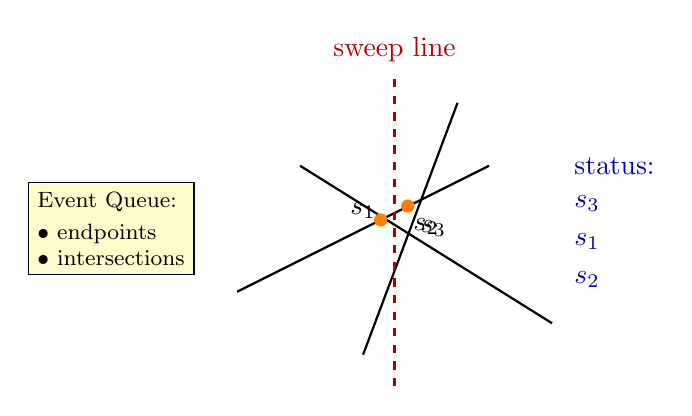
\begin{tikzpicture}[scale=0.8]
  \draw[thick] (0,1)--(4,3) node[midway,above] {$s_1$};
  \draw[thick] (1,3)--(5,0.5) node[midway,above] {$s_2$};
  \draw[thick] (2,0)--(3.5,4) node[midway,right] {$s_3$};
  \draw[red!70!black,thick,dashed] (2.5,-0.5)--(2.5,4.5);
  \node[red!70!black,above] at (2.5,4.5) {sweep line};
  \node[blue!70!black,right] at (5.2,3) {status:};
  \node[blue!70!black,right] at (5.2,2.4) {$s_3$};
  \node[blue!70!black,right] at (5.2,1.8) {$s_1$};
  \node[blue!70!black,right] at (5.2,1.2) {$s_2$};
  \fill[orange] (2.28,2.14) circle (3pt);
  \fill[orange] (2.71,2.36) circle (3pt);
  \node[draw,rectangle,fill=yellow!20,align=left,font=\footnotesize] at (-2,2) {Event Queue:\\[2pt]$\bullet$ endpoints\\$\bullet$ intersections};
\end{tikzpicture}
\caption{Bentley--Ottmann sweep line: the vertical line moves left-to-right. The \emph{status} maintains the vertical order of intersecting segments.}
\label{fig:sweep_line}
\end{figure}


\subsection{Pseudocode}

\begin{algorithm}[htbp]
\caption{Bentley-Ottmann Segment Intersection}
\label{alg:bentley_ottmann}
\begin{algorithmic}[1]
\Function{BentleyOttmann}{segments}
  \State $events \gets \text{PriorityQueue}()$
  \For{$s$ in $segments$}
    \State $events.\text{push}(\text{Event}(s.left, \text{LEFT\_ENDPOINT}, s))$
    \State $events.\text{push}(\text{Event}(s.right, \text{RIGHT\_ENDPOINT}, s))$
  \EndFor
  \State $status \gets \text{BalancedBST}()$
  \State $intersections \gets [\,]$
  \While{$events$ is not empty}
    \State $event \gets events.\text{pop}()$
    \State $p \gets event.point$
    \If{$event.type == \text{LEFT\_ENDPOINT}$}
      \State $s \gets event.segment$
      \State $status.\text{insert}(s, p.x)$
      \State $above, below \gets status.\text{neighbors}(s)$
      \State $\text{CheckIntersection}(s, above, events)$
      \State $\text{CheckIntersection}(s, below, events)$
    \ElsIf{$event.type == \text{RIGHT\_ENDPOINT}$}
      \State $s \gets event.segment$
      \State $above, below \gets status.\text{neighbors}(s)$
      \State $status.\text{remove}(s)$
      \State $\text{CheckIntersection}(above, below, events)$
    \ElsIf{$event.type == \text{INTERSECTION}$}
      \State $s1, s2 \gets event.segments$
      \State $intersections.\text{append}(p)$
      \State $status.\text{swap}(s1, s2)$
      \State $new\_above \gets status.\text{above}(s2)$
      \State $new\_below \gets status.\text{below}(s1)$
      \State $\text{CheckIntersection}(s2, new\_above, events)$
      \State $\text{CheckIntersection}(s1, new\_below, events)$
    \EndIf
  \EndWhile
  \State \Return $intersections$
\EndFunction
\end{algorithmic}
\end{algorithm}

\subsection{Parameters}

\begin{itemize}
\item \textbf{Precision}: Highly sensitive to floating-point errors. Use robust geometric predicates for intersection calculation and segment ordering.
\item \textbf{Degeneracies}: Multiple segments intersecting at the same point or vertical segments require careful handling.
\end{itemize}

\subsection{Complexity}

\begin{itemize}
\item \textbf{Time Complexity}: $O((n + k) \log n)$\index{time complexity!$O((n+k) \log n)$}, where $n$ is the number of segments and $k$ is the number of intersections.
\item \textbf{Space Complexity}: $O(n + k)$ to store the event queue and status structure.
\end{itemize}

\begin{example}[Bentley-Ottmann Trace]\label{ex:bo_trace}
Consider three segments: $s_1 = \{(0,0),(3,3)\}$, $s_2 = \{(0,3),(3,0)\}$, $s_3 = \{(1,0),(1,3)\}$.
\begin{enumerate}
\item Events sorted by $x$: $(0, \text{left}, s_1)$, $(0, \text{left}, s_2)$, $(1, \text{left}, s_3)$, $(3, \text{right}, s_1)$, $(3, \text{right}, s_2)$.
\item After processing $x=0$: Status order (at $x=0^+$) is $s_2$ (above), $s_1$ (below). Check intersection: they meet at $(1.5, 1.5)$: event enqueued.
\item At $x=1$: $s_3$ inserted. Status: $s_2$, $s_3$, $s_1$. Check $s_3$ with $s_2$: they meet at $(1, 2)$: event enqueued. Check $s_3$ with $s_1$: meet at $(1, 1)$: event enqueued.
\item At $x=1$ (intersection $(1,1)$): swap $s_1, s_3$. New neighbors checked.
\item At $x=1$ (intersection $(1,2)$): swap $s_2, s_3$.
\item At $x=1.5$ (intersection $(1.5, 1.5)$): swap $s_1, s_2$.
\item After $x=3$: all segments removed. Three intersection points reported.
\end{enumerate}
\end{example}

\subsection{Usages}

\begin{itemize}
\item \textbf{Map Overlay}: Combining two maps (e.g., roads and counties) to find where they cross.
\item \textbf{Boolean Operations}: Preprocessing for polygon union/intersection.
\item \textbf{CAD/CAM}: Detecting errors in mechanical drawings (e.g., overlapping paths).
\item \textbf{VLSI Design}: Checking for short circuits in circuit board traces.
\item \textbf{Path Planning}: Determining if a path intersects any obstacles.
\end{itemize}

\subsection{Testing and Edge Cases}

\begin{itemize}
\item \textbf{No Intersections}: The algorithm should only process $2n$ events and return empty.
\item \textbf{All segments intersect at one point}: Verify that the event queue handles multiple events at the same location.
\item \textbf{Vertical Segments}: Ensure the ordering logic correctly handles segments with the same $x$-coordinate.
\item \textbf{Collinear Segments}: Overlapping segments on the same line.
\item \textbf{Duplicate Intersections}: Ensure each intersection point is reported only once if multiple segments meet.
\end{itemize}

\subsection{References}

\begin{itemize}
\item Bentley, J. L., \& Ottmann, T. A. (1979). ``Algorithms for reporting and counting geometric intersections''. IEEE Transactions on Computers.
\item Berg, M. de, Cheong, O., Kreveld, M. van, \& Overmars, M. (2008). ``Computational Geometry: Algorithms and Applications''. Springer-Verlag.
\item Wikipedia: Bentley--Ottmann algorithm.
\end{itemize}


\section{Point Location via Trapezoidal Maps}
\label{sec:point_location_trapezoidal}

The point location problem\index{point location} asks, given a planar subdivision and a query point, which face of the subdivision contains that point. It is one of the most fundamental problems in computational geometry, appearing as a subroutine in polygon operations, mesh processing, GIS overlays, and visibility computations. A classical solution is the \emph{trapezoidal map}\index{trapezoidal map} combined with a directed acyclic graph (DAG) search structure, which supports $O(\log n)$ expected query time after $O(n \log n)$ expected preprocessing~\cite{mulmuley1990, seidel1991}. The randomized incremental construction avoids the degeneracy analysis required by deterministic approaches.

\subsection{Definitions}

\begin{definition}[Trapezoid]\label{def:trapezoid}
A \emph{trapezoid}\index{trapezoid} $T$ in a trapezoidal map is a region bounded by two vertical walls (left and right sides), a \emph{top edge} $e_{\text{top}}$, and a \emph{bottom edge} $e_{\text{bot}}$. The left and right boundaries are vertical segments from the bottom edge to the top edge. Each trapezoid is uniquely identified by its left $x$-coordinate, right $x$-coordinate, and the two edges that bound it from above and below.
\end{definition}

\begin{definition}[Trapezoidal Map]\label{def:trapezoidal_map}
Given a set $S$ of $n$ non-intersecting line segments in $\mathbb{R}^2$, the \emph{trapezoidal map} $\mathcal{T}(S)$\index{trapezoidal map} is the subdivision of the plane induced by extending vertical rays from every endpoint of every segment in $S$ upward and downward until they hit a segment or a bounding box. The result is a partition of the plane into $O(n)$ trapezoids.
\end{definition}

\begin{definition}[DAG Search Structure]\label{def:dag_search}
The \emph{DAG search structure}\index{DAG} $D(\mathcal{T})$ is a directed acyclic graph with leaf nodes representing the trapezoids of $\mathcal{T}$ and internal nodes representing \emph{branching queries}. There are two types of internal nodes: \emph{$x$-nodes}\index{$x$-node} (containing a point $p$, branching left if the query has $x < p.x$) and \emph{$y$-nodes}\index{$y$-node} (containing a segment $e = (p_1, p_2)$, branching left if the query is above $e$ and right otherwise). A root-to-leaf path encodes a sequence of decisions that identifies exactly one trapezoid.
\end{definition}

\begin{definition}[$x$-Node]\label{def:x_node}
An \emph{$x$-node}\index{$x$-node} stores a point $p = (p.x, p.y)$. For a query point $q$, the search proceeds to the left child if $q.x < p.x$ and to the right child otherwise. An $x$-node corresponds to an endpoint of a segment.
\end{definition}

\begin{definition}[$y$-Node]\label{def:y_node}
A \emph{$y$-node}\index{$y$-node} stores a segment $e = (p_1, p_2)$ with $p_1.x < p_2.x$. For a query point $q$, the search proceeds to the left child if $q$ lies above $e$ (i.e., the orientation of $(p_1, p_2, q)$ is counter-clockwise) and to the right child otherwise. A $y$-node corresponds to a segment in $S$.
\end{definition}

\subsection{Theory}

\subsubsection*{Construction}

The trapezoidal map is built via a \emph{randomized incremental algorithm}\index{randomized incremental construction}. Starting with a single bounding trapezoid that encompasses the entire input, the segments $s_1, s_2, \ldots, s_n$ are inserted in a uniformly random order. When a new segment $s_k$ is inserted, the existing trapezoids intersected by $s_k$ are located by walking along the trapezoid adjacency graph. Each intersected trapezoid is split into at most four new trapezoids, and the DAG is updated accordingly. Because the insertion order is random, the expected depth of the DAG is $O(\log n)$.

The DAG is a \emph{dag} (directed acyclic graph), not a tree, because multiple internal nodes can share the same child. This sharing is critical: when a segment is inserted and splits an existing trapezoid, the new $x$-node and $y$-node are wired into the DAG at the position of the old leaf, so other paths to that leaf are implicitly updated without duplicating the subtree.

\subsubsection*{Query Algorithm}

To locate a query point $q$, we descend from the root of the DAG:
\begin{enumerate}
\item At an $x$-node with point $p$: go left if $q.x < p.x$, right otherwise.
\item At a $y$-node with segment $e = (p_1, p_2)$: go left if $q$ is above $e$ (counter-clockwise orientation), right otherwise.
\item At a leaf: return the trapezoid stored at that leaf.
\end{enumerate}

The above-below test is performed using the orientation predicate (cross product):
\[
\text{IsAbove}(q, (p_1, p_2)) \iff (p_2.x - p_1.x)(q.y - p_1.y) - (p_2.y - p_1.y)(q.x - p_1.x) > 0.
\]

\begin{theorem}[Trapezoidal Map Complexity]\label{thm:trapezoidal_complexity}
Let $S$ be a set of $n$ non-intersecting line segments in $\mathbb{R}^2$. The randomized incremental trapezoidal map construction with a DAG search structure has expected preprocessing time $O(n \log n)$ and expected space $O(n)$. The expected query time to locate a point in the trapezoidal map is $O(\log n)$, where the expectation is over the random insertion order.
\end{theorem}
\begin{proof}
We analyze the expected size of the search structure using backwards analysis\index{backwards analysis}. Consider the DAG after $k$ segments have been inserted. For any trapezoid $T$ that exists after all $n$ segments are inserted, $T$ was created at some step $k < n$ when the last segment that affects $T$ was inserted. The probability that a particular segment among $\{s_1, \ldots, s_k\}$ is the last to affect $T$ is at most $2/k$ (since $T$ is bounded by at most two segments, and any one of them could be the last inserted among the $k$). Therefore, the expected number of trapezoids created at step $k$ is at most $2$. Summing over $k = 1, \ldots, n$, the total expected number of trapezoids (and hence DAG nodes) is $O(n)$.

The expected depth of a leaf in the DAG is bounded by the expected number of segments whose $x$-nodes or $y$-nodes lie on the root-to-leaf path. By the same backwards analysis, the expected depth of the deepest leaf is $O(\log n)$. Since each level of the DAG is traversed in $O(1)$ time, the expected query time is $O(\log n)$.

The expected total work across all $n$ insertions is $O(n \log n)$ by an amortized argument: at step $k$, the new segment intersects $O(1)$ expected trapezoids, each of which is split in $O(1)$ time, and the DAG update is $O(1)$ per affected node.
\end{proof}

\begin{example}[Trapezoidal Map Construction]\label{ex:trapezoidal_map}
Consider two non-intersecting segments $s_1 = \{(1,1),(3,3)\}$ and $s_2 = \{(2,0),(4,2)\}$ inside a bounding box $[0,5] \times [0,5]$.

\begin{enumerate}
\item \textbf{Initialization}: The bounding trapezoid $T_0$ spans the entire box. The DAG root is a leaf containing $T_0$.

\item \textbf{Insert $s_1$}: The segment $s_1$ splits $T_0$ into trapezoids above and below it. A $y$-node for $s_1$ is created at the root. Its left child is a leaf for the trapezoid above $s_1$; its right child is a leaf for the trapezoid below $s_1$.

\item \textbf{Insert $s_2$}: The segment $s_2$ crosses through the lower trapezoid (the right child of the $s_1$ $y$-node). That trapezoid is split: new $x$-nodes for the endpoints $(2,0)$ and $(4,2)$ are inserted, and additional $y$-nodes for $s_2$ are created. The upper trapezoid (above $s_1$) is unaffected.

\item \textbf{Query for $q = (3, 2.5)$}: Starting at the root ($y$-node for $s_1$): Is $(3, 2.5)$ above $s_1$? Cross product: $(3-1)(2.5-1) - (3-1)(3-1) = 2 \cdot 1.5 - 2 \cdot 2 = -1 < 0$, so $q$ is below $s_1$: go right. Descend through the DAG nodes for the lower region until a leaf is reached, identifying the trapezoid containing $q$.
\end{enumerate}
\end{example}

\subsection{Pseudocode}

The following pseudocode is adapted from the \texttt{TrapezoidalMap} class in the source implementation.

\begin{algorithm}[htbp]
\caption{Trapezoidal Map Query}
\label{alg:trapezoidal_locate}
\begin{algorithmic}[1]
\Function{Locate}{$root$, $q$}
  \State $curr \gets root$
  \While{$curr$ is not a leaf}
    \If{$curr$ is an $x$-node}
      \State $p \gets curr.\text{value}$ \Comment{a point}
      \If{$q.x < p.x$}
        \State $curr \gets curr.\text{left\_child}$
      \Else
        \State $curr \gets curr.\text{right\_child}$
      \EndIf
    \Else \Comment{$y$-node}
      \State $e \gets curr.\text{value}$ \Comment{a segment $(p_1, p_2)$}
      \If{$\text{IsAbove}(q, e)$}
        \State $curr \gets curr.\text{left\_child}$
      \Else
        \State $curr \gets curr.\text{right\_child}$
      \EndIf
    \EndIf
  \EndWhile
  \State \Return $curr.\text{value}$ \Comment{the containing trapezoid}
\EndFunction

\Function{IsAbove}{$q$, $e = (p_1, p_2)$}
  \State \Return $(p_2.x - p_1.x) \cdot (q.y - p_1.y) - (p_2.y - p_1.y) \cdot (q.x - p_1.x) > 0$
\EndFunction
\end{algorithmic}
\end{algorithm}

\begin{algorithm}[htbp]
\caption{Trapezoidal Map Construction (Incremental)}
\label{alg:trapezoidal_build}
\begin{algorithmic}[1]
\Function{TrapezoidalMap}{$bbox$}
  \State $p_1, p_2 \gets bbox$ \Comment{bounding box corners}
  \State $T_0 \gets$ new Trapezoid($p_1, p_2$, top-edge, bottom-edge)
  \State $root \gets$ new node containing $T_0$
  \State $T_0.\text{node} \gets root$
  \State \Return $root$
\EndFunction

\Function{InsertSegment}{$root$, $s_k$}
  \State $T_{\text{start}} \gets$ Locate($root$, $s_k$)
  \State Walk from $T_{\text{start}}$ to the right along adjacent trapezoids intersected by $s_k$
  \For{each intersected trapezoid $T$}
    \State Split $T$ into at most four new trapezoids using $s_k$
    \State Replace the leaf for $T$ in the DAG with a new subtree of $x$-nodes and $y$-nodes
  \EndFor
\EndFunction
\end{algorithmic}
\end{algorithm}

\subsection{Parameters}

\begin{itemize}
\item \textbf{Bounding Box}: A sufficiently large bounding box must be chosen to contain all segments and query points. The bounding box defines the initial trapezoid and the vertical extent of the map.
\item \textbf{Precision}: The orientation predicate \Call{IsAbove}{} uses a cross-product computation. For inputs with nearly collinear segments, a robust predicate with an epsilon tolerance is recommended to avoid numerical instability.
\item \textbf{Randomization}: The insertion order of segments should be uniformly random to guarantee the expected $O(\log n)$ query depth. A poor (adversarial) ordering can lead to $O(n)$ worst-case depth.
\item \textbf{Segment Validity}: The input segments must be non-intersecting (except possibly at shared endpoints). Intersecting segments must be split at their intersection points before building the trapezoidal map.
\end{itemize}

\subsection{Complexity}

\begin{itemize}
\item \textbf{Preprocessing Time}: $O(n \log n)$ expected, where $n$ is the number of segments. Each insertion processes $O(1)$ expected trapezoids, and the walk to find intersected trapezoids is amortized $O(1)$ per segment.
\item \textbf{Space}: $O(n)$ expected. The DAG stores $O(n)$ nodes (both internal and leaf), and each trapezoid stores $O(1)$ data plus adjacency pointers.
\item \textbf{Query Time}: $O(\log n)$ expected. The DAG depth is $O(\log n)$ by backwards analysis, and each level is processed in $O(1)$ time.
\item \textbf{Worst Case}: $O(n)$ query time and $O(n^2)$ space in the worst case (adversarial input ordering), though this is extremely unlikely with randomized construction.
\end{itemize}

\subsection{Usages}

\begin{itemize}
\item \textbf{Planar Subdivision Queries}: Determining which region of a Voronoi diagram, triangulation, or map overlay contains a given point.
\item \textbf{Polygon Operations}: Point location is a subroutine in polygon clipping, union, and intersection algorithms (e.g., Weiler--Atherton).
\item \textbf{Mesh Processing}: Finding which triangle or tetrahedron contains a query point in finite element analysis and computer graphics.
\item \textbf{GIS and Cartography}: Identifying which administrative region, soil type, or land-use zone a GPS coordinate falls within.
\item \textbf{Visibility and Ray Tracing}: Determining the first surface hit by a ray in a 2D scene represented as a planar subdivision.
\item \textbf{Robotics}: Localization within a known map by matching sensor observations to map regions.
\end{itemize}

\subsection{Testing and Edge Cases}

\begin{itemize}
\item \textbf{Point on Segment Boundary}: The orientation predicate may return zero for points exactly on a segment. The implementation should define a consistent convention (e.g., treat collinear as ``not above'').
\item \textbf{Point on Vertical Wall}: Queries on the vertical boundary between two trapezoids should consistently return one of the two trapezoids.
\item \textbf{Empty Map}: A map with no segments should have a single bounding trapezoid; all queries should return that trapezoid.
\item \textbf{Single Segment}: The map should contain exactly two trapezoids (above and below the segment) inside the bounding box.
\item \textbf{Degenerate Segments}: Horizontal or vertical segments should be handled without creating zero-width trapezoids.
\item \textbf{Collinear Endpoints}: Multiple segments sharing an endpoint should produce consistent $x$-node ordering in the DAG.
\item \textbf{Large Input}: Verify that the expected $O(\log n)$ query depth holds empirically for $n > 10{,}000$ segments by measuring average path length.
\end{itemize}

\subsection{References}

\begin{itemize}
\item Mulmuley, K. (1990). ``A fast planar partition algorithm, I''. Journal of Symbolic Computation.
\item Seidel, R. (1991). ``A simple and fast incremental randomized algorithm for computing trapezoidal decompositions and for point location''. Computational Geometry: Theory and Applications.
\item Berg, M. de, Cheong, O., Kreveld, M. van, \& Overmars, M. (2008). ``Computational Geometry: Algorithms and Applications''. Springer-Verlag.
\item Guibas, L. J., \& Sedgewick, R. (1983). ``A dichromatic framework for balanced trees''. IEEE FOCS.
\item Wikipedia: Point location.
\end{itemize}

\section{Point Location in Triangulations (Walking)}
\label{sec:point_location_walking}

\subsection{Overview}
\index{point location!walking}Given a triangulation or tetrahedral mesh
with billions of elements, the \textbf{walking} method locates the simplex
containing a query point by moving across edges (2D) or faces (3D) from a
starting simplex toward the query point. Unlike the trapezoidal map of
Section~\ref{sec:point_location_trapezoidal} (see also the dedicated point
location chapter, Section~\ref{sec:pointloc_triangulations}), which is
restricted to planar subdivisions, walking works directly on a mesh in any
dimension and needs no auxiliary search structure beyond the mesh adjacency
itself. It is the method of choice inside incremental Delaunay construction
(Section~\ref{sec:delaunay_incremental} and \ref{sec:delaunay_edge_flipping})
and for FEM and particle codes that repeatedly query a fixed mesh.

\subsection{Definitions}

\begin{definition}[Visibility Walk]\label{def:visibility_walk}
A \emph{visibility walk} from a starting simplex $\sigma_0$ toward query point
$q$ repeatedly crosses the facet of the current simplex that is
\emph{visible} from $q$: among the facets whose separating hyperplane leaves
$q$ in the opposite half-space, move across the first such facet found. The
walk terminates at a simplex containing $q$.
\end{definition}

\begin{definition}[Jump-and-Walk]\label{def:jump_and_walk}
A \emph{jump-and-walk} first selects a starting simplex $\sigma_0$ using a
spatial index (a grid, k-d tree, or Delaunay tree) that returns a simplex
close to $q$, then walks from $\sigma_0$. The jump makes the walk length
shorter in expectation than a walk from a fixed or random start.
\end{definition}

\begin{definition}[Straight Walk]\label{def:straight_walk}
A \emph{straight walk} from $\sigma_0$ moves, at every step, across the facet
intersected by the line segment from the current position to $q$. It tends to
take fewer steps than a visibility walk but can fail on non-convex or
non-Delaunay meshes; the visibility walk is robust on any triangulation.
\end{definition}

\subsection{Theory}

\begin{theorem}[Visibility Walk Terminates]\label{thm:visibility_walk}
A visibility walk terminates at a simplex containing $q$ on any triangulation
of a convex domain. On a Delaunay triangulation it terminates on any simple
domain~\cite{devillers2002}.
\end{theorem}
\begin{proof}[Proof sketch]
Each crossing strictly decreases the distance from the current simplex to $q$
in the sense of the supporting lines of the crossed facets: the walk cannot
cross the same facet twice, because the crossed hyperplanes separate $q$ from
the already visited simplices. Finiteness follows from the finite number of
facets. The Delaunay case follows because every vertex sees at most one
successive facet, which guarantees progress on non-convex domains as
well~\cite{devillers2002}.
\end{proof}

\begin{theorem}[Expected Walk Length]\label{thm:walk_length}
On a Delaunay triangulation of $n$ points, the expected number of steps of a
walk starting at a random simplex is $O(\sqrt{n})$; with a jump-and-walk whose
starting simplex is chosen near $q$ by a grid or k-d tree, the expected number
of steps is $O(\log n)$ for uniformly distributed points~\cite{devillers2002}.
\end{theorem}
\begin{proof}[Proof sketch]
The expected $O(\sqrt{n})$ bound follows from the fact that the walk crosses
$O(\sqrt{n})$ cells when $n$ points are distributed over a bounded region: the
number of simplices crossed is bounded by the number of simplices intersected
by a segment, which is $O(\sqrt{n})$ in expectation for the Delaunay
triangulation of a uniform set. A spatial-index jump reduces the distance from
the start to the query point, which reduces the expected crossing count to
$O(\log n)$~\cite{devillers2002}.
\end{proof}

\subsection{Pseudocode}

\begin{algorithm}[htbp]
\caption{Locate in a Triangulation by Visibility Walk}
\label{alg:walk_locate}
\begin{algorithmic}[1]
\Function{LocateWalk}{mesh, q, start}
  \State $\sigma \gets start$
  \While{true}
    \State $facet \gets$ first facet of $\sigma$ such that $q$ and $\sigma \setminus facet$ lie on opposite sides of $\operatorname{aff}(facet)$
    \If{no such facet exists} \Comment{$q$ is inside $\sigma$}
      \State \Return $\sigma$
    \EndIf
    \State $\sigma \gets$ neighbor of $\sigma$ across $facet$ \Comment{cross the visible facet}
  \EndWhile
\EndFunction

\Statex

\Function{JumpAndWalk}{mesh, q, grid}
  \State $cells \gets \text{NearestCandidateCells}(q, r, \delta)$ \Comment{grid jump, \cref{sec:fixed_radius_search}}
  \State $\sigma_0 \gets$ a simplex intersecting a cell in $cells$, closest to $q$
  \State \Return \textsc{LocateWalk}(mesh, q, $\sigma_0$)
\EndFunction
\end{algorithmic}
\end{algorithm}

The 3D case is identical with \emph{facets} replaced by the four triangular
faces of a tetrahedron: cross the face whose plane separates $q$ from the
tetrahedron's opposite vertex. In 2D the facet is the single edge separating
$q$ from the opposite vertex.

\subsection{Parameter Selection}
\begin{itemize}
\item \textbf{Start simplex}: for Delaunay construction with spatially sorted
  (Hilbert or Morton) insertion, reuse the simplex found for the previous
  point; for queries, use a grid or k-d tree jump.
\item \textbf{Robust predicates}: use adaptive orientation tests
  (\texttt{orient2d}, \texttt{orient3d}) to avoid looping near
  degeneracies~\cite{shewchuk1997}.
\item \textbf{Tie-breaking}: when $q$ lies exactly on a facet, pick one
  adjacent simplex consistently to avoid infinite loops.
\end{itemize}

\subsection{Complexity}
\begin{itemize}
\item \textbf{Time}: expected $O(\sqrt{n})$ steps from a random start;
  $O(\log n)$ with a grid or k-d tree jump on uniform data.
\item \textbf{Space}: $O(1)$ beyond the mesh itself; the grid jump adds
  $O(n)$.
\item \textbf{No preprocessing}: unlike the trapezoidal map, walking needs no
  auxiliary DAG; it uses only the mesh adjacency.
\end{itemize}

\subsection{Usages}
\begin{itemize}
\item \textbf{Incremental Delaunay construction}: locating the triangle
  containing each inserted point~\cite{bowyer1981,watson1981}.
\item \textbf{FEM post-processing}: reporting which element contains a query
  point or interpolation target.
\item \textbf{Ray tracing and probing} of volumetric (tetrahedral) meshes.
\end{itemize}

\subsection{Testing and Edge Cases}
\begin{itemize}
\item \textbf{Termination}: compare against the trapezoidal map location
  (Section~\ref{sec:point_location_trapezoidal}) for 2D on the same mesh;
  results must agree.
\item \textbf{Boundary points}: queries exactly on an edge or vertex must
  return a consistent simplex.
\item \textbf{Non-convex meshes}: use the visibility walk (not the straight
  walk) and verify termination on meshes with concavities.
\item \textbf{Large input}: measure average walk length over $n$ queries and
  confirm it matches the theoretical $O(\log n)$ or $O(\sqrt{n})$ growth.
\item \textbf{Counterexample checks}: the straight walk can fail on
  non-Delaunay meshes; assert the visibility walk is always used there.
\end{itemize}

\subsection{References}
\begin{itemize}
\item Devillers, O. (2002). ``The Delaunay hierarchy''. International Journal
  of Foundations of Computer Science.
\item Bowyer, A. (1981). ``Computing Dirichlet tessellations''. The Computer
  Journal.
\item Watson, D. F. (1981). ``Computing the $n$-dimensional Delaunay
  tessellation''. The Computer Journal.
\item Shewchuk, J. R. (1997). ``Adaptive precision floating-point arithmetic
  and fast robust geometric predicates''. Discrete \& Computational Geometry.
\end{itemize}
